\begin{flushleft}
{\Huge Hyfsvisor\\}
\vspace{1 cm}
{\Large
När huvudrätten lider mot sitt slut och gästerna är mätta och belåtna
kungör toastmastern hyfs. Vid hyfs sjunges en av
hyfsvisorna nedan, varpå all vätska i glasen drickes upp. Detta sker för att bereda plats för punsch eller dylik söt dryck till
efterrätten. Efter hyfsandet serveras efterrätten med kaffe och avec.}
\end{flushleft}

\vspace{2cm}
\begin{center}
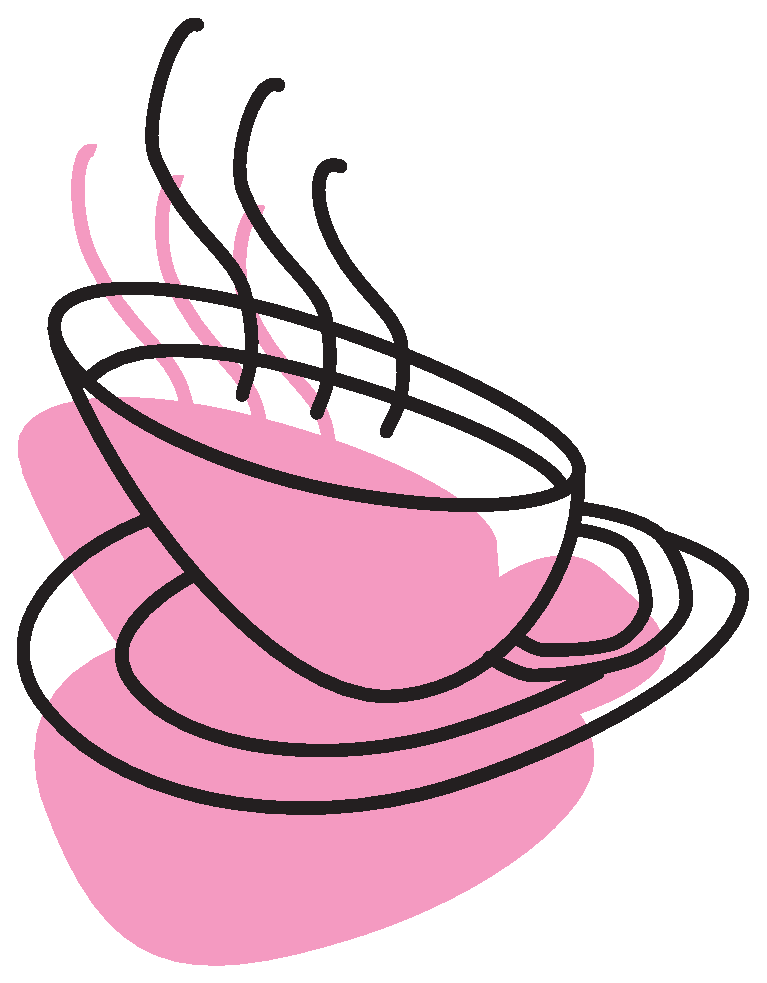
\includegraphics[width=6cm]{bilder/43.eps}
\end{center}
\newpage

\begin{song}{Härjarevisan}{harjarevisan}
\mel{Gärdebylåten\\ur Lundaspexet Djingis Kahn}
\begin{vers}
Liksom våra fäder \\
vikingarna i Norden\\
drar vi riket runt\\
och super oss under borden.\\
Brännvinet har blitt ett elixir\\
för kropp såväl som själ.\\
Känner du dig liten\\
och ynklig på jorden,\\
växer du med supen\\
och blir stor uti orden,\\
slår dig för ditt håriga bröst\\
och blir en man från hår till häl.\\
\end{vers}
\begin{vers}
Ja, nu skall vi ut och härja: \\
supa och slåss och svärja,\\
bränna röda stugor, slå små\\
barn och säga fula ord.\\
Med blod ska vi stäppen färga.\\
Nu änteligen lär jag\\
kunna dra nån riktigt nytta av min\\
Hermodskurs i mord\\
\end{vers}
\newp
\begin{vers}
Hurra nu ska man äntligen \\
få röra på benen\\
hela stammen jublar\\
och det spritter i grenen.\\
Tänk att än en gång\\
få spränga fram på Brunte i galopp.\\
Din doft o kära Brunte\\
är trots brist i hygienen\\
för en vild mongol\\
minst lika ljuv som syrenen.\\
Tänk att på din rygg\\
få rida runt i stan och spela topp!\\
\end{vers}
\begin{vers}
Ja nu ska vi ut och härja... \\
\end{vers}
\begin{vers}
Ja mordbränder är klämmiga, \\
ta fram fotogenen.\\
Och eftersläckningen\\
tillhör just de fenomenen\\
inom brandmansyrket som jag\\
tycker är nån nytta med.\\
Jag målar för mitt inre upp\\
den härliga scenen;\\
blodrött mitt i brandgult,\\
ej ens prins Eugen en\\
lika mustig vy kan måla,\\
ens om han målade med sked.\\
\end{vers}
\begin{vers}
Ja nu ska vi ut och härja...\\
\end{vers}
\end{song}

\begin{song}{Kalmarevisan}{kalmarevisan}
\begin{vers}
För uti Kalmare stad\\
ja där finns det ingen kvast förrän lördagen.\\
\end{vers}
\begin{vers}
//: När som bonden kommer hem\\
då går bondekvinnan ut ://\\
och är ful i sin trut\\
Hej dick! Hej dack!\\
Jag slog i, och vi drack!\\
Hej dickomdickomdack!\\
Hej dickomdickomdack!\\
För uti Kalmare stad,\\
ja där finns det ingen kvast förrän lördagen.\\
\end{vers}
\begin{vers}
//: Var är pengarna du fått?\\
Jo, dom har jag supit opp! ://\\
uppå Kalmare slott.\\
Hej dick . . .\\
\end{vers}
\begin{vers}
//: Jag skall mäla dig an\\
för vår kronbefallningsman ://\\
så att du skall få skam\\
Hej dick . . .\\
\end{vers}
\begin{vers}
//: Kronbefallningsmannen vår\\
satt på krogen i går ://\\
och var full som ett får.\\
Hej dick . . .\\
\end{vers}
\end{song}









